% Options for packages loaded elsewhere
\PassOptionsToPackage{unicode}{hyperref}
\PassOptionsToPackage{hyphens}{url}
\PassOptionsToPackage{dvipsnames,svgnames,x11names}{xcolor}
%
\documentclass[
  10pt,
  dvipsnames,enabledeprecatedfontcommands]{scrartcl}
\usepackage{amsmath,amssymb}
\usepackage{lmodern}
\usepackage{iftex}
\ifPDFTeX
  \usepackage[T1]{fontenc}
  \usepackage[utf8]{inputenc}
  \usepackage{textcomp} % provide euro and other symbols
\else % if luatex or xetex
  \usepackage{unicode-math}
  \defaultfontfeatures{Scale=MatchLowercase}
  \defaultfontfeatures[\rmfamily]{Ligatures=TeX,Scale=1}
\fi
% Use upquote if available, for straight quotes in verbatim environments
\IfFileExists{upquote.sty}{\usepackage{upquote}}{}
\IfFileExists{microtype.sty}{% use microtype if available
  \usepackage[]{microtype}
  \UseMicrotypeSet[protrusion]{basicmath} % disable protrusion for tt fonts
}{}
\usepackage{xcolor}
\usepackage{graphicx}
\makeatletter
\def\maxwidth{\ifdim\Gin@nat@width>\linewidth\linewidth\else\Gin@nat@width\fi}
\def\maxheight{\ifdim\Gin@nat@height>\textheight\textheight\else\Gin@nat@height\fi}
\makeatother
% Scale images if necessary, so that they will not overflow the page
% margins by default, and it is still possible to overwrite the defaults
% using explicit options in \includegraphics[width, height, ...]{}
\setkeys{Gin}{width=\maxwidth,height=\maxheight,keepaspectratio}
% Set default figure placement to htbp
\makeatletter
\def\fps@figure{htbp}
\makeatother
\setlength{\emergencystretch}{3em} % prevent overfull lines
\providecommand{\tightlist}{%
  \setlength{\itemsep}{0pt}\setlength{\parskip}{0pt}}
\setcounter{secnumdepth}{5}
\newlength{\cslhangindent}
\setlength{\cslhangindent}{1.5em}
\newlength{\csllabelwidth}
\setlength{\csllabelwidth}{3em}
\newlength{\cslentryspacingunit} % times entry-spacing
\setlength{\cslentryspacingunit}{\parskip}
\newenvironment{CSLReferences}[2] % #1 hanging-ident, #2 entry spacing
 {% don't indent paragraphs
  \setlength{\parindent}{0pt}
  % turn on hanging indent if param 1 is 1
  \ifodd #1
  \let\oldpar\par
  \def\par{\hangindent=\cslhangindent\oldpar}
  \fi
  % set entry spacing
  \setlength{\parskip}{#2\cslentryspacingunit}
 }%
 {}
\usepackage{calc}
\newcommand{\CSLBlock}[1]{#1\hfill\break}
\newcommand{\CSLLeftMargin}[1]{\parbox[t]{\csllabelwidth}{#1}}
\newcommand{\CSLRightInline}[1]{\parbox[t]{\linewidth - \csllabelwidth}{#1}\break}
\newcommand{\CSLIndent}[1]{\hspace{\cslhangindent}#1}
%\documentclass{article}

% %packages
 \usepackage{booktabs}
\usepackage{subcaption}
\usepackage{multirow}
\usepackage{colortbl}
\usepackage{graphicx}
\usepackage{longtable}
\usepackage{ragged2e}
\usepackage{etex}
%\usepackage{yfonts}
\usepackage{marvosym}
\usepackage[notextcomp]{kpfonts}
\usepackage{nicefrac}
\newcommand*{\QED}{\hfill \footnotesize {\sc Q.e.d.}}
\usepackage{floatrow}
%\usepackage[titletoc]{appendix}
%\renewcommand\thesubsection{\Alph{subsection}}

\usepackage[textsize=footnotesize]{todonotes}
\newcommand{\ali}[1]{\todo[color=gray!40]{#1}}
\newcommand{\mar}[1]{\todo[color=blue!40]{#1}}
\newcommand{\raf}[1]{\todo[color=olive!40]{#1}}
%\linespread{1.5}
\newcommand{\indep}{\!\perp \!\!\! \perp\!}


\setlength{\parindent}{10pt}
\setlength{\parskip}{1pt}


%language
\usepackage{times}
\usepackage{t1enc}
%\usepackage[utf8x]{inputenc}
%\usepackage[polish]{babel}
%\usepackage{polski}




%AMS
\usepackage{amsfonts}
\usepackage{amssymb}
\usepackage{amsthm}
\usepackage{amsmath}
\usepackage{mathtools}

\usepackage{geometry}
 \geometry{a4paper,left=35mm,top=20mm,}


%environments
\newtheorem{fact}{Fact}



%abbreviations
\newcommand{\ra}{\rangle}
\newcommand{\la}{\langle}
\newcommand{\n}{\neg}
\newcommand{\et}{\wedge}
\newcommand{\jt}{\rightarrow}
\newcommand{\ko}[1]{\forall  #1\,}
\newcommand{\ro}{\leftrightarrow}
\newcommand{\exi}[1]{\exists\, {_{#1}}}
\newcommand{\pr}[1]{\mathsf{P}(#1)}
\newcommand{\cost}{\mathsf{cost}}
\newcommand{\benefit}{\mathsf{benefit}}
\newcommand{\ut}{\mathsf{ut}}

\newcommand{\odds}{\mathsf{Odds}}
\newcommand{\ind}{\mathsf{Ind}}
\newcommand{\nf}[2]{\nicefrac{#1\,}{#2}}
\newcommand{\R}[1]{\texttt{#1}}
\newcommand{\prr}[1]{\mbox{$\mathtt{P}_{prior}(#1)$}}
\newcommand{\prp}[1]{\mbox{$\mathtt{P}_{posterior}(#1)$}}



\newtheorem{q}{\color{blue}Question}
\newtheorem{lemma}{Lemma}
\newtheorem{theorem}{Theorem}



%technical intermezzo
%---------------------

\newcommand{\intermezzoa}{
	\begin{minipage}[c]{13cm}
	\begin{center}\rule{10cm}{0.4pt}



	\tiny{\sc Optional Content Starts}
	
	\vspace{-1mm}
	
	\rule{10cm}{0.4pt}\end{center}
	\end{minipage}\nopagebreak 
	}


\newcommand{\intermezzob}{\nopagebreak 
	\begin{minipage}[c]{13cm}
	\begin{center}\rule{10cm}{0.4pt}

	\tiny{\sc Optional Content Ends}
	
	\vspace{-1mm}
	
	\rule{10cm}{0.4pt}\end{center}
	\end{minipage}
	}
%--------------------






















\newtheorem*{reply*}{Reply}
\usepackage{enumitem}
\newcommand{\question}[1]{\begin{enumerate}[resume,leftmargin=0cm,labelsep=0cm,align=left]
\item #1
\end{enumerate}}

\usepackage{float}

% \setbeamertemplate{blocks}[rounded][shadow=true]
% \setbeamertemplate{itemize items}[ball]
% \AtBeginPart{}
% \AtBeginSection{}
% \AtBeginSubsection{}
% \AtBeginSubsubsection{}
% \setlength{\emergencystretch}{0em}
% \setlength{\parskip}{0pt}






\usepackage[authoryear]{natbib}

%\bibliographystyle{apalike}



\usepackage{tikz}
\usetikzlibrary{positioning,shapes,arrows}

\ifLuaTeX
  \usepackage{selnolig}  % disable illegal ligatures
\fi
\IfFileExists{bookmark.sty}{\usepackage{bookmark}}{\usepackage{hyperref}}
\IfFileExists{xurl.sty}{\usepackage{xurl}}{} % add URL line breaks if available
\urlstyle{same} % disable monospaced font for URLs
\hypersetup{
  pdftitle={``Weight of Evidence, Evidential Completeness and Accuracy''},
  pdfauthor={Rafal Urbaniak and Marcello Di Bello},
  colorlinks=true,
  linkcolor={Maroon},
  filecolor={Maroon},
  citecolor={Blue},
  urlcolor={blue},
  pdfcreator={LaTeX via pandoc}}

\title{``Weight of Evidence, Evidential Completeness and Accuracy''}
\author{Rafal Urbaniak and Marcello Di Bello}
\date{}

\begin{document}
\maketitle

\hypertarget{motivations}{%
\section{Motivations}\label{motivations}}

\hypertarget{balance-vs.-weight}{%
\subsection{Balance vs.~weight}\label{balance-vs.-weight}}

Suppose we want to represent our uncertainty about a proposition in
terms of a single probability that we assign to it. It is not too
difficult to inspire the intuition that this representation does not
capture an important dimension of how our uncertainty connects with the
evidence we have or have not obtained. In a 1872 manuscript of
\emph{The Fixation of Belief} (W3 295) C. S. Peirce gives an example
meant to do exactly that.

\begin{quote} When we have drawn a thousand times, if about half have been white, we have great confidence in this result. We now feel pretty sure that, if we were to make a large number of bets upon the color of single beans drawn from the bag, we could approximately insure ourselves in the long run by betting each time upon the white, a confidence which would be entirely wanting if, instead of sampling the bag by 1000 drawings, we had done so by only two.
\end{quote}

\noindent The objection is not too complicated. Your best estimate of
the probability of \(W=\)`the next bean will be white' is .5 if half of
the beans you have drawn randomly so far have been white, no matter
whether you have drawn a thousand or only two of them. But this means
that expressing your uncertainty about \(W\) by locutions such as ``my
confidence in \(W\) is .5' does not capture this intuitively important
distinction.

Similar remarks can be found in Peirce's 1878
\emph{Probability of Induction}. There, he also proposes to represent
uncertainty by at least two numbers, the first depending on the inferred
probability, and the second measuring the amount of knowledge obtained;
as the latter, Peirce proposed to use some dispersion-related measure of
error (but then suggested that an error of that estimate should also be
estimated and so, so that ideally more numbers representing errors would
be needed).

Peirce himself did not call this the weight of evidence (and in fact,
used the phrase rather to refer to the balance of evidence, W3 294)
{[}CITE KASSER 2015{]}. However, his criticism of such an oversimplified
representation of uncertainty anticipated what came to be called weight
of evidence by Keynes in his 1921 \emph{A Treatise on Probability}:

\begin{quote}
As the relevant evidence at our disposal increases, the magnitude of the
probability of the argument may either increase or decrease, according as the new knowledge strengthens the unfavourable or the favourable evidence; but something seems to have increased in either case,—we have a more substantial basis upon which to rest our conclusion. I express this by saying that an accession of new evidence increases the weight of an argument. New evidence will sometimes decrease the probability of an argument but it will always increase its `weight.' (p. 71)
\end{quote}

\noindent The key point is the same {[}CITE LEVI 2001{]}: the balance of
probability alone cannot characterize all important aspects of
evidential appraisal. Keynes also considered measuring weight of
evidence in terms of the variance of the posterior distribution of a
certain parameter, but was quite attached to the idea that weight should
increase with new information, even if the dispersion increase with new
evidence {[}TP 80-82{]}, and so he proposed only a very rough sketch of
a positive sketch. Moreover, as he was uncertain how a measure of weight
should be incorporated in further decision-making, the was skeptical
about the practical significance of the notion. {[}TP 83{]}

But what is this positive sketch? On one hand, Keynes {[}TP 58-59{]}
connects the notion of weight with relevance. Call evidence \(E\)
relevant to \(X\) given \(K\) just in case
\(\mathsf{Pr}(X\vert K \wedge E) \neq \mathsf{Pr}(X \vert K)\).\footnote{
  Keynes also uses a slightly more convoluted notion of relevance to
  avoid equally strong items of opposite evidence turning out to be
  irrelevant (this objection has also been brought up by {[}COHEN 1986
  TWELVE{]}). The more complex version is that a proposition \(E_1\) is
  relevant to \(X\) given \(K\) just in case it entails a proposition
  \(E_2\) such that
  \(\pr{X\vert K \wedge E_2} \neq \mathsf{Pr}(X \vert K)\). {[}COHEN
  1986 TWELVE{]} complaints that this still runs into difficulties.
  Ignore \(K\), take an irrelevant proposition \(Z\). It entails
  \(Z\vee X\) and \(\pr{Z \vee X\vert X \wedge E}=1\). Now, by Bayes'
  theorem we have
  \(\pr{X \vert E \wedge (Z \vee X)} = \frac{\pr{X \vert E}\times \pr{Z \vee X \vert X \wedge E}}{\pr{Z \vee X \vert E}} = \frac{\pr{X \vert E}}{\pr{Z \vee X \vert E}}\).
  If the denominator differs from 1, the result differs from the
  numerator. We will ignore such difficulties, as they are not of key
  importance for the development of this chapter.} One postulate than
can be found in the \emph{Treatise} {[}TP 84{]} is:\footnote{RUNDE 1990
  283 suggests Keynes allows for weight of evidence to decrease when new
  evidence increases the range of alternatives, but this is based on
  Keynes' claim that weight is increased when the number of alternatives
  is reduced, and Keynes does not directly say anything about the
  possibility of an increase of the number of alternatives.}

\begin{tabular}{lp{11cm}}
(Monotonicity) & If $E$ is relevant to $X$ given $K$, where $K$ is background knowledge, $V(X\vert K \wedge E) > V(X\vert K)$, where $V$ is the weight of evidence.
\end{tabular}

{[}RUNDE 1990, 280{]} suggests that Keynes at some point calls weight
the completeness of information. This however, is a bit hasty, as Keynes
only says that
\emph{the degree of completeness of the information on which a probability is based does seem to be relevant, as well as the actual magnitude of the probabiltiy, in making practical decisions}.
As later on we will argue that it is actually useful to distinguish
evidential weight (how much evidence do we have?) and evidential
completeness (do we have all the evidence that we would expect in a
given case?), we rather prefer to extract a more modest postulate:

\begin{tabular}{lp{11cm}}
(Completeness) & If $E_1$ and $E_2$ are relevant items of evidence, and $E_2$ is (in a sense to be discussed) more complete than $E_1$,  $V(X\vert K \wedge E_2) > V(X\vert K \wedge E_1)$.
\end{tabular}

\noindent If we conceptualize \(E_2\) being complete and \(E_1\) being
incomplete as \(E_2\) being a maximal relevant conjunction of relevant
claims one of which is \(E_1\), (Completeness) follows from
(Monotonicity).

Similar requirements seem to be inspired by the urn example. We put them
in two forms, a weaker and a stronger one.

\begin{tabular}{lp{11cm}}
(Weak increase) & In cases analogous to the urn example, the weight obtained by a larger sample is higher, if the frequencies in the samples remain the same.\\
(Strong increase) & In cases analogous to the urn example, the weight obtained by a larger sample is higher.
\end{tabular}

Now, some requirements on how weight of evidence is related to the
balance of probability. For one thing, Keynes insists that new
(relevant) evidence might decrease probability but will always increase
weight {[}TP 77{]}. Since (Monotonicity) already captures the idea that
weight will always increase, here we extract the other part of the
claim:

\begin{tabular}{lp{11cm}}
(Possible decrease) & It is possible that   $V(X\vert K \wedge E) > V(X\vert K)$ while $\pr{X \vert K \wedge E} <  \pr {X\vert K}$.
\end{tabular}

Clearly, Keynes also endorsed the following two requirements of a very
similar form:

\begin{tabular}{lp{11cm}}
(Possible increase) & It is possible that   $V(X\vert K \wedge E) > V(X\vert K)$ while $\pr{X \vert K \wedge E} >  \pr {X\vert K}$. \\
(Possibly no change ) & It is possible that   $V(X\vert K \wedge E) > V(X\vert K)$ while $\pr{X \vert K \wedge E} =  \pr {X\vert K}$.
\end{tabular}

Interestingly, Keynes for quite a few years did not attempt to provide
anything close to a formal explication of the notion, and did not spend
too much time studying the issue. Various reasons for this has been
proposed the literature, a prominent one {[}CITE FEDUZI 2010{]} being
that from the decision-theoretic perspective no clear stopping rule
emerged as to whether the evidence is weighty enough to make a decision.
\todo{Should I talk about other theories here, or should we leave it as is without getting into interpretative details.}
Later on we will see a sort of revival---some ideas later developed by
Keynes has been used to explicate the notion of weight formally, and we
will take a closer look at this proposal. \todo{REF section}

\hypertarget{examples-and-informal-desiderata}{%
\subsection{Examples and informal
desiderata}\label{examples-and-informal-desiderata}}

\begin{itemize}
\item
  Go over Nance in particular, some other sources?
\item
  first check for completeness, then evaluate
\item
  what do you mean: are there items of relevant evidence that you could
  reasonably obtain
\item
  destroyed?
\end{itemize}

\hypertarget{monotonicity-of-weight}{%
\subsubsection{Monotonicity of weight}\label{monotonicity-of-weight}}

Before we move on, let us ponder whether (Monotonicity) is actually
desirable. Is it always the case, as some formulations from Keynes would
suggest, that any item of relevant of evidence, when obtained, leads to
a higher weight of evidence?

Here are two examples from {[}WEATHERSON 2002{]}, one qualitative, one
quantitative.\todo{CITE B. Weatherson. Keynes, uncertainty and interest rates. Cambridge Journal of Eco-
nomics, 26 (1): 47-62, 2002.]} First. you are playing poker and wonder
if one of the other players, Lydia, has a straight flush (five cards of
sequential rank in the same suite). There are 40 possible straight flush
hands out of 2,958,960 possible hands, so you estimate the probability
of this event to be \(\nicefrac{40}{2,958,960}\). But then you look at
her facial expressions, listen to her tone of voice, past bluffing
behavior, and this makes you more confused about the issue. It seems,
obtaining this additional information diluted your original calculated
first stab at the problem. Second. You are drawing from an urn with 10
blue and 90 black lottery tickets. Your initial assessment of the
probability of drawing a blue ticket is .1. Then, you learn that the
proportion of the tickets at the top is somewhere between .2 and 1. You
acquired new evidence, but your evidence became imprecise. In both
cases, it seems intuitive that the weight of evidence should decrease,
as the evidence becomes less telling.

\hypertarget{hamers-weight-of-evidence}{%
\subsection{Hamer's weight of
evidence}\label{hamers-weight-of-evidence}}

\hypertarget{goods-weigh-of-evidence-and-the-information-value}{%
\subsection{Good's weigh of evidence and the information
value}\label{goods-weigh-of-evidence-and-the-information-value}}

One notion in the vicinity also called \emph{weight of evidence} has
been introduced by Good {[}CITE PROBABILITY AND THE WEIGHING OF EVIDENCE
1950{]}. Let \(W(H:E)\) be the Good's weigh of evidence in favor of
\(H\) provided by \(E\) (if we want to explicitly conditionalize on some
background knowledge \(K\), we write \(W(H:E\vert K)\)). One assumption
about \(W\) taken by Good is as
follows:\todo{pays attention to different values of different items of evidence, which is better than just counting or supersets}

\begin{tabular}{lp{11cm}}
(Function) & ``It is natural to assume that $W(H:E)$ is some function of $\pr{E\vert H}$ and of $\pr{E\vert \neg H}$, say $f[\pr{E\vert H}, \pr{E \vert \neg H}]$. I cannot see how anything can be relevant to the weight of evidence other than the probability of the evidence given guilt and the probability given innocence.'' [cite Good 1985 p 250]
\end{tabular}

The other two are:

\begin{tabular}{lp{11cm}}
(Independence) & $\pr{H\vert E} $ should depend only on the weight of evidence and on the prior: $\pr{H \vert E} = g[W(H:e), \pr{H}]$.\\
(Additivity)  & $W(H: E_1 \wedge E_2)  = W(H:E_1) + W(H:E_2 \vert E_1)$
\end{tabular}

\noindent The three conditions can be simultaneously satisfied by only
one function (up to a constant factor), which leads to Good's definition
of weight of evidence:\footnote{To be fair, logarithms of the ratio of
  posterior odds to prior odds have been used Jeffrey in 1936,
  {[}CITE{]} and the use of logarithm to ensure additivity has been
  suggested by Turing {[}CITE 1950 o 63{]}. Good's measure differs from
  Jeffrey's by taking the ratio of likelihoods rather than odds. In
  fact, the former ratio is identical to
  \(\nicefrac{O(H\vert E)}{O(H)}\), the ratio of conditional odds of
  \(H\) to the prior odds of \(H\).} \begin{align*}
W(H:E) & = \log \frac{\pr{E \vert H}}{\pr{E\vert \neg H}}
\end{align*}

The natural question that arises is the extent to which Good's weight
satisfies the desiderata related to Keynes' notion of weight. First, let
us think about weight increase with sample size. If in an experiment the
observations \(E_1, \dots, E_K\) are independent given \(H\) and
independent given \(\neg H\), the resulting joint likelihood is the
result of the multiplication of the individual likelihoods, and so the
resulting joint weight is the result of adding the individual weights.

For example, suppose a die is selected at random from a hat containing
nine fair dice and one loaded die with the chance \(\nicefrac{1}{3}\) of
obtaining a six. The initial uniform distribution gives you weight of
evidence for the die being loaded of \(log_{10}(.1)\), that is -1 (Good
and Turing would say, it is -10 db). Now, every time you toss it and
obtain a six, you gain
\(log_{10}(\frac{\nicefrac{1}{3}}{\nicefrac{1}{6}})= log_{10}(2)\), that
is 0.30103, and every time you toss it and obtain something else, the
weight changes by
\(log_{10}(\frac{\nicefrac{2}{3}}{\nicefrac{5}{6}})= log_{10}(.8)\),
that is -0.09691. Let us inspect the weights in db (that is, multiplied
by 10) for all possible outcomes of up to 20 tosses (Figure
\ref{fig:goodWeight}).

\begin{figure}

\begin{center}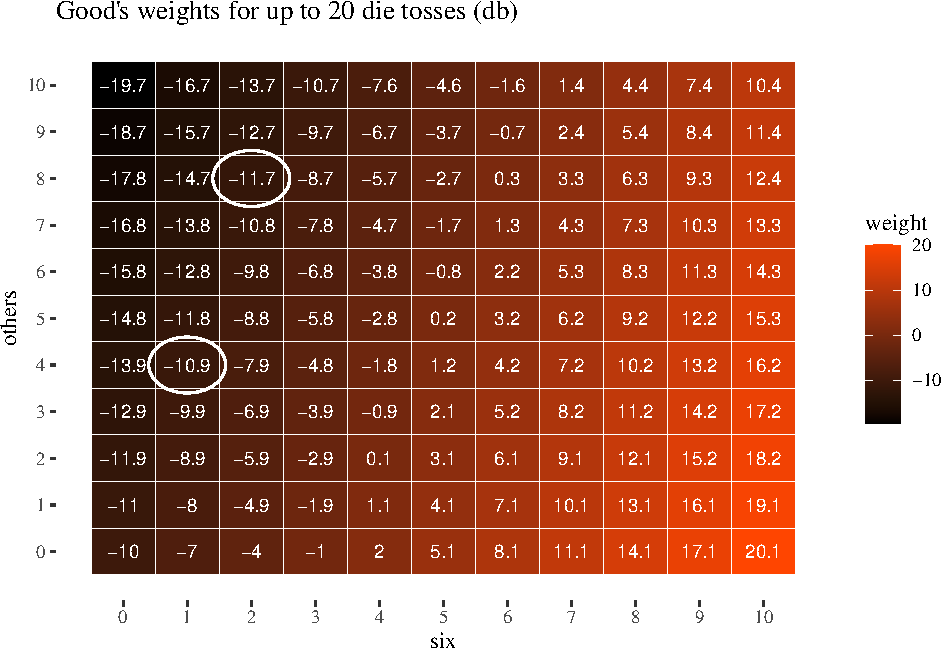
\includegraphics[width=1\linewidth]{imprecision_weight_files/figure-latex/goodWEights-1} \end{center}
\caption{Good's weights in dbs, rounded, for all possible outcomes of up to 20 tosses of a die randomly selected from 10 dice nine of which were fair, and one is \nicefrac{1}{3} loaded towards six. $H=$`the die is loaded'.}
\label{fig:goodWeight}
\end{figure}

Two facts are notable. (1) Weight can drop with sample size: for
instance the weight for 4 others and 5 sixes is 1.2db, and it is .2db
for 5 others and 5 sixes. (2) Weight can drop while the sample size
increases even if the proportion of sixes remains the same. For
instance, if none of the observations are sixes, the weights go from -10
to -19.7 as the sample size goes from 0 to 10. Less trivially, the
observation of one six in five leads to weight of -10.9, while the
observation of two sixes in ten tosses leads to weight -11.7. That is,
(Monotonicity), (Completeness), (Weak increase) and (Strong increase)
all fail for Good's measure.

Moreover, there is a conceptual difficulty in the neighborhood. Suppose
you are trying to ascertain the bias \(\theta\) of a coin, but you do
not restrict yourself to two hypotheses as in the dice example, but
rather initially take any bias to be equally likely. For each particular
hypothesis \(\theta = x\) and any set of observations \(E\) you can use
the binomial distribution to calculate \(\pr{E \vert \theta = x}\). But
to deploy Good's definition, you also need
\(\pr{E \vert \theta \neq x}\), which is less trivial, as now you have
to integrate to calculate the expected probability of the evidence given
an infinite array of possible values of \(y\). Suppose you have no
problem calculating such items. Now imagine you observe 10 heads in 20
tosses. The question `how weighty is the evidence' makes no sense here,
as Good's weight needs a hypothesis (and its negation) to be plugged in.
For this reason, in such a situation, we can at best talk about a
continuum of Good's weights, one for each particular value of
\(\theta\).

\begin{itemize}
\item
  compare to pointwise mutual information
\item
  evaluate in light of the desiderata
\end{itemize}

\hypertarget{weight-and-completeness}{%
\subsection{Weight and completeness}\label{weight-and-completeness}}

A question similar to ``how weighty is the evidence'' is ``how complete
is it''? These are conceptually different: the former asks about how
much information pertinent to a given hypotheses the evidence provides,
or, about the amount of evidence relevant to that hypothesis, the latter
seems to suggest a comparison to some ideal list of what such items
would be needed for the evidence to be complete. While we think that
these notions, albeit related, should be clearly distinguished, the
distinction has not always been made clearly in the literature, starting
with Keynes himself, who suggested that in their evaluation of the
evidence an agent should consider ``the degree of completeness of the
information upon which a probability is based.'' {[}TP
p.~345{]}\todo{REF}

This picture of ideal-list-of-evidence-relative notion of weight has
been explored by {[}CITE FEDUZI 2010{]}. \todo{CITE NANCE HERE?} Let us
first present the view following {[}CITE FEDUZI 343{]}, \(\Omega\)
stands for the set of all items of possible evidence relevant for
estimating the probability of the hypothesis \(H\). Let \(K\) be the
agent's knowledge, the set of items of evidence already obtained by the
agent, \(K \subseteq \Omega\). Then her relevant ignorance is
\(I = \Omega \setminus K\).

Then, Feduzi, following {[}CITE RUNDE 1990{]}, proposes to define the
weight of information \(E\) provides about \(H\), \(V(H/E)\) as follows:
\begin{align} \tag{Vdiv}  V(H/E) & = \frac{K}{K+I}.\end{align}
\noindent While literally it does not make sense to divide sets by sets,
we might charitably interpreting Feduzi as using \(\Omega, K\) and \(I\)
the symbols ambiguously, standing for both the sets of items of
evidence, and the amount of relevant information that the sets contain.
The obvious difficulty is that it is not a successful explication (at
least not yet), as we are not told how to get \(K\) and \(K+I\) as
numerical values to be used in the division. But however we get them,
let us see whether (Vdiv) can result in any insights.

First, one advantage of the completeness approach is that the resolution
of the stopping problem is more or less automatic: the agent should make
the decision if the evidence is complete, and should collect more
evidence if it is not. Later on, when discussing Nance's approach to the
notion, we will see a complication: obtaining further evidence might be
practically unfeasible, and so it makes sense to distinguish ideal
completeness from reasonable completeness and base the practical
stopping rule on the former. For now, we put this complication aside.

Second, it might be the case that obtaining further evidence while
providing more information results in the decrease of weight. Here is an
example illustrating this due to Feduzi {[}CITE 345{]}. Joan in her
research tries to establish who is the most quoted author in the
literature on decision theory under ambiguity. \(\Omega\) is the set of
all \(n\) papers (though of as items of evidence \(E_1, \dots, E_n\)).
\(K_0\) contains the \(m\) papers that Joan inspected so far
(\(E_1, \dots, E_m\), \(m<n\). \(I_0\) is the set of papers she did not
look at yet, \(\Omega = K_0 \cup I_0\). However, Joan is aware only of a
part of \(\Omega\), the papers in the field she believes exist, \(S\).
Thus, her objective ignorance, \(I_0\), and her subjective ignorance,
\(I_S = S- K\), diverge, as she underestimates the amount of papers that
she has not yet encountered. Joan's assessment of weight is going to be
\(\nicefrac{K}{K+I_s}\). Say Joan formulates a hypothesis, \(H\):
``Ellsberg is the most highly cited author in the ambiguity literature''
and that she is quite confident that the papers she had not looked at
yet would not significantly affect the probability of \(H\). She thinks
she has read enough, say \(\pr{H \vert K} = .7\) and \(V(H/K) = .8\).
Then, she looks at another paper, somewhat increasing \(K\), but that
paper contains reference to many papers she has not heard of in journals
that she has not heard of, thus increasing her estimation of \(S\) quite
a lot--- the ultimate impact of the new evidence is a drop in weight as
the denominator in (Vdiv) will grow much more than the numerator. Thus,
(Monotonicity) \todo{check crossref} can fail on this approach.

However, even putting the conceptual difference between weight and
completeness that we have already mentioned aside, there are concerns
about using degrees of completeness as our explication of the notion of
weight of evidence.

To start with, we have not really explicated the notion of the amount of
evidence employed in (Vdiv). Sure, we could simply count propositions.
One simple strategy, to be used if we do not want to use (Vdiv) would be
to simply count the relevant propositions included in the
evidence---this would validate (Monotonicity) \todo{check crossref}.
Another strategy along these lines would be to assign sizes to sets of
propositions and use these as numbers in (Vdiv), invalidating
(Monotonicity) in the process. Either way, the strategy is not viable,
as it is too syntax-sensitive. Different propositions, intuitively, can
contain hugely different amount of nevertheless relevant information
\todo{is this trivial or do we need an example?}, and the individuation
of propositions is too arbitrary a matter to take such an approach
seriously. On one hand, without some measure of assigning numerical
values to sets of evidence, we have no way to deploy (Vdiv). On the
other hand, if we could meaningfully assign numbers expressing the
``amount of evidence'' prior to any application of (Vdiv), there are no
clear reasons why we should take these number to express weights of
evidence, especially given the second concern with the completeness
approach.

So the second difficulty is that on this approach the weight of evidence
becomes very sensitive not only to what the actual evidence is, but also
to what an ideal evidence in a given case should be. unless as clear and
epistemologically principled guidance as to how to formulate such ideal
lists is available, this seems to open a gate to arbitrariness. Change
of awareness of one's own ignorance, without any major chance to the
actual evidence obtained, might lead to overconfidence or
under-confidence in one's judgment. Moreover, it is not clear how
disagreement about weight arising between agents not due to evidential
differences, but rather due to differences in their list of ideal items
of evidence should be adjudicated.

\hypertarget{skyrms-and-resilience}{%
\subsection{Skyrms and resilience?}\label{skyrms-and-resilience}}

\begin{itemize}
\tightlist
\item
\item
  relation to law Davidson Pargetter 1986, perhaps Nance, who else?
\end{itemize}

\hypertarget{evidential-probability-and-weight}{%
\subsection{Evidential probability and
weight}\label{evidential-probability-and-weight}}

{[}PEDDEN 2018{]} \todo{REF} follows a suggestion from {[}KYBURG
1961{]}\todo{REF Kyburg. Probability and the Logic of Rational Belief. Wesleyan University Press, Mid-
dletown Connecticut, 1961 and H. E. Kyburg and C. M. Teng. Uncertain Inference. Cambridge University Press, Cam-
bridge, 2001.} He proposed using the degree of imprecision of the
intervals in his probability system called Evidential Probability (EP).
The key idea in EP is that evidential probabilities should be imprecise,
and so accordingly an evidential probability function \(\mathsf{EP}\) is
of the form \(\mathsf{EP}(H \vert E \wedge K) = [x,y]\), where the
right-hand is the closed interval expressing the objective degree of
support that \(E\wedge K\) provide for \(H\).

How is this interval to be determined, though? Kyburg's proposal is the
following, if the hypothesis is about a single object \(o\) and a
predicate \(P\). For the reference classes to which \(o\) is known to
belong and for which \(K\) contains frequency information (possibly
imprecise, in the interval form) for objects with \(P\), enumerate the
corresponding frequency statements, \(r_1, \dots, r_n\). Now, you are
facing a reference class problem. Apply sequentially the following
rules:

\begin{tabular}{lp{10cm}}
(Sharpening by richness) & If $r_j$ conflicts with $r_i$ and $r_i$ has been obtained from a marginal distribution while $r_j$ from a full joint distribution, ignore $r_i$. 
\end{tabular}

As the formulation might be somewhat cryptic, let us illustrate the
recommendation with an
example.\todo{make sure these examples are better made sense of the HOP way!}

\begin{tabular}{lp{10cm}}
(Richness example) &suppose you are drawing a card from one of two decks of cards, $H:=$ `you will draw the Ace of Spades'. You know that Deck 1 is a regular deck, and Deck 2 is a regular Deck with the Ace of Spades removed. First you toss a fair die and use Deck 1 if the die lands on 1 or 2, and use Deck 2 otherwise. You have at least two frequencies to consider:
\begin{itemize}
\item The frequency of Aces of Spades in the total number o cards ($\nicefrac{1}{103}$), which is your marginal-distribution-based-probability.
\item The one obtained by using the information about the die, and about the frequencies in the decks. There is probability $\nicefrac{1}{3}$ of using Deck 1 which is the only deck containing the card, in which the probability of drawing it is $\nicefrac{1}{52}$, so the probability to be used is $\nicefrac{1}{3}\nicefrac{1}{52}= \nicefrac{1}{156}$.
\end{itemize}
\end{tabular}

One can easily observe that \(\nicefrac{1}{103}\) simply is not the
probability of drawing the Ace of Spades in the setup. After all, we are
not drawing a random card from the joint decks, but have to factor in
the uneven probabilities of the decks being chosen, and once we do so,
the correct probability is \(\nicefrac{1}{156}\). The second strategy is
this:

\begin{tabular}{lp{10cm}}
(Sharpening by specificity) & If among the remaining intervals $r_j$ conflicts with $r_i$ and $r_j$ is a proper subset of $r_i$, choose $r_j$ over $r_i$.
\end{tabular}

\noindent This mirrors the idea that one should use more specific
information. The third rule is:

\begin{tabular}{lp{10cm}}
(Sharpening by precision) & If there is a single interval that is a proper sub-interval  of every other interval, this is the evidential probability. Otherwise, the evidential probability is the shortest possible cover of these intervals.
\end{tabular}

With this system in the background, {[}PEDDEN 2018 681{]} proposes the
following definition of the weight of the argument for \(H\) given \(E\)
and \(K\), where \(\mathsf{EP}(H \vert E \wedge K) = [x,y]\):
\begin{align}
\tag{WK} & \mathsf{WK(H\vert E\wedge K)} & = 1 - (y-x)
\end{align} That is, the weight of the evidence is the spread of the
evidential probability, transformed to scale between 0 and 1, reaching 1
when the spread is 0 and 0 when the spread is 1.

How is this approach to be applied to examples such as the one by C. S.
Peirce (recall: drawing balls with replacement from an urn, with
observed frequency of white balls .5, in one scenario the sample size is
1000 in another it is 2)?

{[}PEDDEN 2018 686{]} proposes the following analysis, of an example
analogous to that by Peirce. You are drawing from an urn full of black
and red beans (the proportion is unknown). First, abbreviations:

\begin{tabular}{lp{10cm}}
$H$ & $49.5-50.5\%$ of the beans are red. \\
$E_1$ & 2 sampled beans are red. \\
$E_2$ & 3000 sample beans are red. 
\end{tabular}

\noindent Further, imagine you have enough information to calculate that
between \(2\%\) and \(100\%\) of two-fold samples of any large finite
population will be matching samples, that is they will match the
population with a margin of error of \(1\%\). Then
\(\mathsf{EP}(H \vert E_1 \wedge K) = [.02, 1]\). Similarly, Pedden
invites us to suppose that we can calculate the relative frequency of
3000-fold samples that match any large finite population within a margin
of error of \(1\%\) to somewhere between \(72.665\%\) and \(100\%\), so
accordingly \(\mathsf{EP}(H \vert E_2 \wedge K) = [.72665, 1]\). Then,
the corresponding values of \(\mathsf{WK}\) are .02 and .72665 (this is
because in both cases \(y =1\) and \(1 - (1 -x) = x\)).

What are we to make of this? Are imprecise probabilities promising when
it comes to the explication of weight of evidence? Some progress has
been made, but note the following limitations.

\begin{itemize}
\item
  The edges of the intervals are what contributes to \textsf{WK}. They
  are highly sensitive to the choice of the margin of error, but what
  margin of error to choose and why remains a mystery, and what margin
  of error has been chosen does not function anywhere in the
  \(\mathsf{EP}\) representation of uncertainty.
\item
  Relatedly, it may easily happen that for two different distributions
  the \(1\%\) intervals will be identical while the 78\%\$ intervals
  will not. Such differences will obviously not be captured by the 1\%
  margin of error intervals.
\item
  The calculations of such intervals might be easy for simple
  combinatorial cases, but it is far from obvious how similar intervals
  are to be obtained for more complicated real-life cases. Emphatically,
  classical statistical confidence intervals are not ranges within which
  the true parameter lies with a certain probability (and if you
  interpret confidence intervals this way, you behave as if you were
  running a Bayesian reasoning with a uniform prior, which is often
  unjustified and prone to over-fitting).
\end{itemize}

Before we abandon the idea, though, let us know that over the last 30
years we have observed a revival of imprecise probabilities, and so it
is only fair that we should take its most recent versions for a ride.
Hence our next interest: imprecise probabilism, its motivations, the
difficulties it runs into.

\hypertarget{imprecise-probabilities-and-weight}{%
\subsection{Imprecise probabilities and
weight}\label{imprecise-probabilities-and-weight}}

The point of departure for imprecise probabilism (\textsf{IP}) is the
precise probabilism (\textsf{PP}), which we are already familiar with.
On the latter view, a rational agent's uncertainty is to be represented
as a single probability measure. \textbf{Imprecise probabilism}, in
contrast with PP, holds that an agent's credal stance towards a
hypothesis \(H\) is to be represented by means of a set of probability
measures, called a representor, \(\mathbb{P}\), rather than a single
measure \(\mathsf{P}\). The idea is that the representor should include
all and only those probability measures which are compatible with this
evidence. For instance, if an agent knows that the coin is fair, their
credal stance would be captured by \(\{\mathsf{P}\}\), where
\(\mathsf{P}\) is simply a probability measure which assigns \(.5\) to
\(H\). If, on the other hand, the agent knows nothing about the coin's
bias, their stance would rather be represented by means of the set of
all probabilistic measures, as none of them is excluded by the available
evidence. Note that on IP it is not the case that the set represents
admissible options and the agent can legitimately pick any precise
measure from the set. Rather, the agent's credal stance is essentially
imprecise and has to be represented by means of the whole
set.\footnote{For the development of IP see (Fraassen, 2006; Gärdenfors
  \& Sahlin, 1982; Joyce, 2005; Kaplan, 1968; Keynes, 1921; Levi, 1974;
  Sturgeon, 2008; Walley, 1991), (Bradley, 2019) is a good source of
  literature.} The literature contains an array of arguments for IP. Let
us take a look at the main ones.

\begin{itemize}
\item
  \textsf{PP} does not seem appropriately evidence-responsive,
  especially when evidence is limited. Following \textsf{PP}, in
  Peirce's example, the agent's uncertainty about \(W:=\)``the next
  drawn ball is going to be white' is \(.5\) no matter whether you have
  drawn two balls one of which was white, or a thousand balls, five
  hundred of which were white.
\item
  Indifference is not sensitive to sweetening (improving the chances of
  \(H\) only slightly), while \textsf{PP} predicts such sensitivity. For
  instance, if you do not know what the bias of a coin is, learning that
  it now has been slightly modified to increase the probability of heads
  by .001 will still leave you unwilling to bet on heads in a bet that
  would've been fair if the actual chance of \(H\) was .5 and not .001.
\item
  \textsf{PP} has problems representing complete lack of knowledge.
  Suppose you start tossing the coin starting with knowing only that the
  coin bias is in \([0,1]\) and then observe the outcome of ten tosses,
  half of which turn out to be heads. This is some evidence for the real
  bias being around .5. How do you represent your stances before and
  after the observations? If you deploy the principle of insufficient
  evidence, you start with \(\mathsf{P}_0(H)=.5\) and end with
  \(\mathsf{P}_1(H)=.5\), as if nothing changed. If you do not deploy
  the principle of insufficient evidence, what do you do?
\item
  \textsf{PP} has problems with formulating a sensible method of
  probabilistic opinion aggregation Stewart \& Quintana (2018). A
  seemingly intuitive constraint is that if every member agrees that
  \(X\) and \(Y\) are probabilistically independent, the aggregated
  credence should respect this. But this is hard to achieve if we stick
  to PP (Dietrich \& List, 2016). For instance, a \emph{prima facie}
  obvious method of linear pooling does not respect this. Consider
  probabilistic measures \(p\) and \(q\) such that
  \(p(X) = p(Y) = p(X\vert Y) = 1/3\) and
  \(q(X) = q(Y) = q(X\vert Y) = 2/3\). On both measures, taken
  separately, \(X\) and \(Y\) are independent. Now take the average,
  \(r=p/2+q/2\). Then \(r(X\cap Y) = 5/18 \neq r(X)r(Y)=1/4\).
\end{itemize}

One key difference between Kyburg's \textsf{EP} and \textsf{IP} is that
on the latter we use sets of probability measure instead of intervals.
This makes the approach not only more general (as now, for instance, the
resulting probabilities of a proposition in question do not have to form
a closed interval), but also provides a more general and less
idiosyncratic picture of learning from evidence, that is a a natural
extension of the classical Bayesian approach. When faced with new
evidence \(E\) between time \(t_0\) and \(t_1\), RA's representor should
be updated point-wise, running the standard Bayesian updating on each
probability measure in the representor:
\begin{align*} \label{eq:updateRepresentor}
\mathbb{P}_{t_1} = \{\mathsf{P}_{t_1}\vert \exists\, {\mathsf{P}_{t_0} \!\in  \mathbb{P}_{t_0}}\,\, \forall\, {H}\,\, \left[\mathsf{P}_{t_1}(H)=\mathsf{P}_{t_0}(H \vert E)\right] \}.
\end{align*}

\hypertarget{troubles-with-imprecise-probabilism}{%
\subsection{Troubles with imprecise
probabilism}\label{troubles-with-imprecise-probabilism}}

\begin{itemize}
\item
  \textsf{IP} has no means of distinguishing the situation in which you
  are about to toss a coin whose bias is either .4 or .6., and the one
  in which you are about to toss a coin whose bias is either .4 or .6,
  and bias .4 is three times more likely than .6.
\item
  \textsf{IP} give wrong comparison predictions (Rinard, 2013). Suppose
  you know of two urns, \textsf{GREEN} and \textsf{MYSTERY}. You are
  certain \textsf{GREEN} contains only green marbles, but have no
  information about \textsf{MYSTERY}. A marble will be drawn at random
  from each. You should be certain that the marble drawn from
  \textsf{GREEN} will be green (\(G\)), and you should be more confident
  about this than about the proposition that the marble from
  \textsf{MYSTERY} will be green (\(M\)). In line with how lack of
  information is to be represented on \textsf{IP}, for each
  \(r\in [0,1]\) your representor contains a \(\mathsf{P}\) with
  \(\pr{M}=r\). But then, it also contains one with \(\pr{M}=1\). This
  means that it is not the case that for any probability measure
  \(\mathsf{P}\) in your representor, \(\mathsf{P}(G) > \mathsf{P}(M)\),
  that is, it is not the case that RA is more confident of \(G\) than of
  \(M\). This is highly counter-intuitive.
\item
  While \textsf{IP}, does not seem to have a problem reprentic complete
  lack of information, the way it is represented makes agents
  susceptible to belief inertia (Levi, 1980). Recall the example in
  which you start tossing a coin starting with knowing only that the
  coin bias is in \([0,1]\) and then observe the outcome of ten tosses,
  half of which turn out to be heads. On \textsf{IP} your initial credal
  state is to be modeled by the set of all possible probability measures
  over your algebra of propositions . Once you observe the ten results,
  each particular measure from your initial representor gets updated to
  a different one that assigns a value closer to .5 to Heads, but also
  each measure in your original representor can be obtained by updating
  some other measure in your original representor by updating on the
  evidence. Thus, if you are to update your representor point-wise, you
  will end up with the same representor set.
\end{itemize}

\hypertarget{a-second-order-approach-to-uncertainty}{%
\subsection{A second-order approach to
uncertainty}\label{a-second-order-approach-to-uncertainty}}

\hypertarget{information-theoretic-weight-of-evidence}{%
\subsection{Information-theoretic weight of
evidence}\label{information-theoretic-weight-of-evidence}}

\hypertarget{completeness-tends-to-improve-weight}{%
\subsection{Completeness tends to improve
weight}\label{completeness-tends-to-improve-weight}}

\hypertarget{weight-tends-to-improve-accuracy}{%
\subsection{Weight tends to improve
accuracy}\label{weight-tends-to-improve-accuracy}}

Here is a question asked by {[}COHEN 1986 TWELVE p.~276{]}: is it worth
while knowing the weight of an argument without knowing its probability?
In our terminology, questions inspired by Cohen's are: what's the point
of weight considerations if we already have the distributions? Can
weights be put to use if we do not have the distributions?

\hypertarget{literature-to-discuss}{%
\section{Literature to discuss}\label{literature-to-discuss}}

Kasser, 2016, Two Conceptions of Weight of Evidence in Peirce's
Illustrations of the Logic of Science {[}COVERED{]}

Feduzi, 2010, On Keynes's conception of the weight of evidence COVERED

Cohen 1986, Twelve Questions about Keynes's Concept of Weight
{[}COVERED{]}

Pedden, William 2018, Imprecise probability and the measurement of
Keynes' weight of arguments {[}GET BACK TO INERTIA, DILUTION ETC.{]}

Levi 2011, the weight of argument {[}DOWNLOADED{]}

Skyrms 1977 resiliency, propensities {[}DOWNLOADED{]}

Skyrms causal necessity, chapter on resilience {[}DOWNLOAD{]}

Synthese 186 (2) 2012, volume on Keynesian weight {[}CHECKED, NOT MUCH
ON WEIGHT ACTUALLY, NO NEED TO READ{]}

Good, weight of evidence, survey

Good, PROBABILITY AND THE WEIGHING OF EVIDENCE

David Hamer, Probability, anti-resilience, and the weight of expectation
{[}READ{]}

William Peden, Imprecise Probability and the Measurement of Keynes's
``Weight of Arguments''

Runde, Keynesian Uncertainty and the weight of arguments
{[}DOWNLOADED{]}

Weatherson, 2002, Keynes, uncertainty and interest rates
{[}DOWNLOADED{]}

Jeffrey M. Keisler, Value of information analysis: the state of
application

Edward C. F. Wilson, A Practical Guide to Value of Information Analysis

Joyce JM (2005) How probabilities reflect evidence.

Kyburg. Probability and the Logic of Rational Belief. Wesleyan
University Press, Middletown Connecticut, 1961

H. E. Kyburg and C. M. Teng. Uncertain Inference. Cambridge University
Press, Cam- bridge, 2001.

\hypertarget{refs}{}
\begin{CSLReferences}{1}{0}
\leavevmode\vadjust pre{\hypertarget{ref-bradley2019imprecise}{}}%
Bradley, S. (2019). {Imprecise Probabilities}. In E. N. Zalta (Ed.),
\emph{The {Stanford} encyclopedia of philosophy} ({S}pring 2019).
\url{https://plato.stanford.edu/archives/spr2019/entries/imprecise-probabilities/};
Metaphysics Research Lab, Stanford University.

\leavevmode\vadjust pre{\hypertarget{ref-Dietrich2016pooling}{}}%
Dietrich, F., \& List, C. (2016). Probabilistic opinion pooling. In A.
Hajek \& C. Hitchcock (Eds.), \emph{Oxford handbook of philosophy and
probability}. Oxford: Oxford University Press.

\leavevmode\vadjust pre{\hypertarget{ref-Elkin2018resolving}{}}%
Elkin, L., \& Wheeler, G. (2018). Resolving peer disagreements through
imprecise probabilities. \emph{Noûs}, \emph{52}(2), 260--278.
\url{https://doi.org/10.1111/nous.12143}

\leavevmode\vadjust pre{\hypertarget{ref-VanFraassen2006vague}{}}%
Fraassen, B. C. V. (2006). Vague expectation value loss.
\emph{Philosophical Studies}, \emph{127}(3), 483--491.
\url{https://doi.org/10.1007/s11098-004-7821-2}

\leavevmode\vadjust pre{\hypertarget{ref-Gardenfors1982unreliable}{}}%
Gärdenfors, P., \& Sahlin, N.-E. (1982). Unreliable probabilities, risk
taking, and decision making. \emph{Synthese}, \emph{53}(3), 361--386.
\url{https://doi.org/10.1007/bf00486156}

\leavevmode\vadjust pre{\hypertarget{ref-joyce2005probabilities}{}}%
Joyce, J. M. (2005). How probabilities reflect evidence.
\emph{Philosophical Perspectives}, \emph{19}(1), 153--178.

\leavevmode\vadjust pre{\hypertarget{ref-Kaplan1968decision}{}}%
Kaplan, J. (1968). Decision theory and the fact-finding process.
\emph{Stanford Law Review}, \emph{20}(6), 1065--1092.

\leavevmode\vadjust pre{\hypertarget{ref-keynes1921treatise}{}}%
Keynes, J. M. (1921). \emph{A treatise on probability, 1921}. London:
Macmillan.

\leavevmode\vadjust pre{\hypertarget{ref-Levi1974ideterminate}{}}%
Levi, I. (1974). On indeterminate probabilities. \emph{The Journal of
Philosophy}, \emph{71}(13), 391. \url{https://doi.org/10.2307/2025161}

\leavevmode\vadjust pre{\hypertarget{ref-Levi1980enterprise}{}}%
Levi, I. (1980). \emph{The enterprise of knowledge: An essay on
knowledge, credal probability, and chance}. MIT Press.

\leavevmode\vadjust pre{\hypertarget{ref-Rinard2013against}{}}%
Rinard, S. (2013). Against radical credal imprecision. \emph{Thought: A
Journal of Philosophy}, \emph{2}(1), 157--165.
\url{https://doi.org/10.1002/tht3.84}

\leavevmode\vadjust pre{\hypertarget{ref-Stewart2018pooling}{}}%
Stewart, R. T., \& Quintana, I. O. (2018). Learning and pooling, pooling
and learning. \emph{Erkenntnis}, \emph{83}(3), 1--21.
\url{https://doi.org/10.1007/s10670-017-9894-2}

\leavevmode\vadjust pre{\hypertarget{ref-Sturgeon2008grain}{}}%
Sturgeon, S. (2008). Reason and the grain of belief. \emph{No{û}s},
\emph{42}(1), 139--165. Retrieved from
\url{http://www.jstor.org/stable/25177157}

\leavevmode\vadjust pre{\hypertarget{ref-walley1991statistical}{}}%
Walley, P. (1991). \emph{Statistical reasoning with imprecise
probabilities}. Chapman; Hall London.

\end{CSLReferences}

\end{document}
